\section{Frontend}
\label{sc:frontend}
Na rozdíl od backendu, frontend moduly se nijak neinicializují, jelikož vystavují už hotové komponenty a GraphQL mutace a query. Na druhou stranu frontend dělá více, než jen skládání mutací a query do jednoho endpointu. Proto následující sekce probírají podrobněji důležité a specifické aspekty aplikace. Funkce jako správa uživatelů nejsou ničím specifické, a tedy i přesto, že jsou implementované, nemá smysl se nimi zabývat v~rámci této práce.

\subsection{Server Side Rendering}
\label{ss:ssr}
Největším oříškem, co se týče nastavení projektu a výběru technologií, je funkce zvaná \acrfull{ssr}. Některé projekty se tímto vůbec nezabývají a to hlavně jelikož to pro ně nemá moc přínos, ale na druhou stranu to přidá hodně práce. Hlavní důvody, proč implementovat \acrshort{ssr} jsou dva, první je \acrshort{seo} optimalizace a druhá je optimalizace tzv. \acrfull{fcp}, tedy času od začátku požadavku než uživatel uvidí něco užitečného. Tato \emph{užitečná} informace může být i třeba jen zobrazení načítání, ale je lepší uživateli zobrazit nejprve načítání a až pak interaktivní aplikaci, než čekat stejnou dobu na interaktivní aplikaci a mezitím mít zobrazenou bílou stránku.

Pro funkci \acrshort{ssr} však musíme mít další Node.js server, který obsluhuje http požadavky. Tento server pro vybrané, nebo pro všechny cesty vyrenderuje aplikaci a vrátí html soubor, které již danou aplikaci obsahuje. Pokud takto obsluhuje jen některé cesty, tak pro zbylé vrací standardní \emph{prázdný} html soubor, bílou stránku, a render aplikace pak nechává na klientovi. Pokud byla aplikace renderovaná na serveru, tak klient musí provést ještě jeden krok, zvaný hydratace, který celou aplikaci projde, vytvoří virtuální DOM strukturu, se kterou potom vnitřně pracuje a aplikaci oživí.

Tato aplikace implementuje \acrshort{ssr} kvůli~\nameref{NP03}. Aplikace bez \acrshort{ssr} vrací klientovi html soubor s~špatně nastavenou hlavičkou a web crawleři většinou nemají podporu JavaScriptu, takže ani nikdy neuvidí vyrenderovanou aplikaci. Správné nastavení hlavičky zajišťuje knihovna \emph{react-helmet}. který při renderování na straně serveru extrahuje title a meta tagy, které jsou následně poslané v~hlavičce výsledku.

\subsection{Lokalní správa stavu aplikace}
\label{ss:local_state_management}
Aplikace potřebuje mít nějakou správu globálního stavu, a to hlavně aby komponenty mohli reagovat na to jestli je uživatel přihlášený, nebo ne. Pro tuto funkcionalitu se běžně v~aplikacích používá velmi oblíbená knihovna \emph{redux}. Správu lokálního stavu však umožňuje i knihovna Apollo Client, která již je v~aplikaci kvůli provolívání backend serveru.

Apollo Client přistupuje ke správě lokálního stavu aplikace odlišně, než jiné knihovny. Místo upravováního nějakého globálního storu pomocí funkcí, reducerů nebo něčeho podobného, je lokální stav upravovaný GraphQL mutacemi a čten pomocí query. Tyto mutace a query se však musí nějak odlišit od normálních požadavků a z~toho důvodu jsou označeny anotací \mintinline{javascript}{@client}. Takový požadavek Apollo Client zachytí a zpracuje pomocí lokálních resolverů. Tato data jsou ukládány a čteny z~stejné paměti, kterou Apollo Client používá pro ukladání cache požadavků.

\subsection{CSS in JS}
\label{ss:css_in_js}
Je mnoho možností, jak přistupovat k~stylování komponent, čisté CSS, preprocesory SASS či LESS a CSS modules. Další možností je CSS in JS, které kombinuje všechny uvedené možnosti a navíc zlehčuje interakci s~JavaScriptem. Místo standardních souborů dedikovaných jen pro stylování, jsou styly psané v~rámci javascriptových nebo typescriptových souborů ve formě funkcí, objektů nebo template literals. Dvě nejpoužívanější knihovny poskytující tuto funkcionalitu jsou \href{https://styled-components.com/}{\emph{styled-components}} a \href{https://emotion.sh/}{\emph{emotion}}. Emotion má menší velikost balíčku, lepší podporu \acrshort{ssr}, je rychlejší \cite{shehet_2020_css}, lépe optimalizovaný pro \gls{tree shaking}. Volba právě této knihovny umožnila rychlý a jednoduchý vývoj s~podporou více vzhledů aplikace.

\subsection{Code splitting}
\label{ss:code_splitting}
Code splitting je metoda rozdělení sestavené aplikace na více souborů. Jde o~optimalizaci ve formě zmenšení prvotního načítání. Aplikace je teda rozdělena na části, které se načítají postupně, jak uživatel prochází aplikací. Při první návštěvě se tedy ke klientovi stahuje soubor \emph{main.js}, který obsahuje nutné části aplikace a pak další soubor, podle toho jakou stránku navštívil. Při přechodu na další stránku se donačte skript pro tu danou stránku. Tím se docílí snížení čas \acrshort{fcp}. Navíc některé stránky, třeba administrátorské, běžný uživatel nikdy neuvidí, tak nepotřebuje stahovat jejich skripty.

Možností jak docílit efektivního rozdělování kódu je několik \cite{facebookinc_2018_codesplitting}. První možností je na úrovni webpacku, což ale z~dlouhodobého hlediska není udržitelné. Dále tuto funkcionalitu poskytuje \emph{React.lazy} a \emph{Suspense}, který ale zatím nepodporuje \acrshort{ssr} \cite{facebookinc_2018_codesplitting}. Poslední možnosti jsou externí knihovny, jako například \href{https://github.com/jamiebuilds/react-loadable}{\emph{react-loadable}}. Tato knihovna s~minimem nastavení umožňuje rozdělovat kód buď podle cest, nebo přímo komponent a její použití je velmi jednoduché, viz~\ref{code:code_splitting}

\begin{figure}[h!]
    \centering
    \begin{minted}{javascript}
// standardní import komponenty
import HomePage from './homepage';

const LoadableHopePage = Loadable({
    // import funkce
    loader: () => import('./homepage'),
    // komponenta zobrazená místo té načítané v průběhu načítaní
    loading: Loading,
});
    \end{minted}
    \caption{Code splitting pomocí react-loadable}
    \label{code:code_splitting}
\end{figure}

\subsection{Ukládání písní}
\label{ss:song_saving}
Ukládání textů písní a akordů je netriviální záležitost. Je potřeba ukládat texty písní přesně na řádky a k~nim akordy na správné pozice. Tento problém je vyřešen tak, že píseň má text uložený ve speciálním formátu. Tento formát je pole řádků a každý řádek se skládá z~textu a pole objektů, které reprezentují akord a jeho pozice od začátku řádku. Následně je text písně zobrazen neproporciálním písmem a akordy nad ním, také neproporciálním písmem. Tím jsou zaručené jednotné odstupy písmen a akordy jsou tedy na správných místech.

\subsection{Vykreslování akordů}
\label{ss:chords_render}
Komponenta akordů je další specifická funkce této aplikaci, proto musela být vytvořena na míru. Alternativní možností bylo aplikaci připojit na API\footnote{https://ukulele-chords.com/api}, které vrací vykreslené akordy. Tento proces by práci sice zjednodušil, ale vygenerované obrázky jsou černobílé, což barevně nezapadá do konceptu aplikace a navíc nepodporují více barevných schémat. Z~toho důvodu je tato komponenta implementovaná ručně. Také to je jediná komponenta, která pracuje přímo s~grafikou. Vzhledem k~jednoduchosti této grafiky a požadavku na co nejvyšší rychlost, tak je vykreslování implementováno přímo pomocí \href{https://developer.mozilla.org/en-US/docs/Web/API/Canvas_API}{Canvas API} a není pro to využita žádná knihovna. Tento přístup přinesl lehce konfigurovatelnou komponentu, která se škáluje bez ztrát a podporuje více barevných schémat, na rozdíl od rastrového obrázku z~API.

\begin{figure}
    \centering
    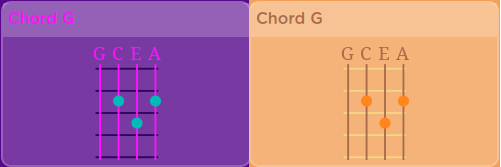
\includegraphics[width=0.9\textwidth]{assets/g_chord.png}
    \caption{Příklad komponenty akordu}
    \label{fig:g_chord}
\end{figure}